\documentclass[aps,prl,twocolumn,showpacs,superscriptaddress,groupedaddress]{revtex4}  % for review and submission
%\documentclass[aps,prl,preprint,groupedaddress]{revtex4-1}

%\documentclass[aps,preprint,showpacs,superscriptaddress,groupedaddress]{revtex4}  % for double-spaced preprint
\usepackage{graphicx}  % needed for figures
\usepackage{dcolumn}   % needed for some tables
\usepackage{bm}        % for math
\usepackage{amssymb}   % for math

% avoids incorrect hyphenation, added Nov/08 by SSR
%hyphenation{ALPGEN}

\begin{document}

% The following information is for internal review, please remove them for submission
\widetext
\leftline{Version xx as of \today}
\leftline{Primary authors: MIT, NTU}
\leftline{To be submitted to PRL}

\title{Measurements of two-particle correlations in $e^+e^-$ collisions at 91 GeV with ALEPH archived data}
\author{Yen-Jie Lee}
\author{Anthony Badea}
\author{Austin Baty}
\author{Christopher McGinn}
\author{Gian Michele Innocenti}
\author{Jesse Thaler}
\author{Michael Peters}
\affiliation{Massachusetts Institute of Technology, Cambridge, USA}%
\author{Tzu-An Sheng}
\author{Paoti Chang}
\affiliation{National Taiwan University, Taipei, Taiwan}%
\author{Marcello Maggi}
\affiliation{INFN Sezione di Bari, Bari, Italy}%

\date{\today}


\begin{abstract}
The first measurements of two-particle angular correlations for charged particles emitted in $e^+e^-$ collisions at a center-of-mass energy of 91 GeV are presented. The archived data are collected with the ALEPH detector at LEP. The correlation functions are measured over a broad range of pseudorapidity and azimuthal angle of the charged particles. Those results are compared to predictions from the PYTHIA event generator. In contrast to the results from high charged particle multiplicity nucleon-nucleon, nucleon-nucleus and nucleus-nucleus collisions, where long-range correlations with a large pseudorapidity gap are observed, no significant enhancement of long-range correlations is observed with respect to PYTHIA predictions, which do not include additional final state interactions of the outgoing partons. 
\end{abstract}

\pacs{}
\maketitle

Two-particle correlations in high-energy collisions provide valuable information for characterizing Quantum Chromodynamics and have been studied previously for a broad range of collision energies in proton-proton (pp)~\cite{Khachatryan:2010gv,Aad:2015gqa}, proton-nucleus (pA)~\cite{CMS:2012qk,Abelev:2012ola,Aad:2012gla}, deutron-nucleus (dA)~\cite{Adare:2013piz}, and nucleus-nucleus (AA)~\cite{Aamodt:2010pa,Chatrchyan:2012wg} collisions. Such measurements can elucidate the underlying mechanism of particle production and reveal possible collective effects resulting from the high particle densities accessible in these collisions.
Studies of two-particle angular correlations are typically performed the using the two-dimensional $\Delta\eta-\Delta\phi$ correlation functions, where $\Delta\phi$ is the difference in the azimuthal angle $\phi$ between the two particles and $\Delta\eta$ is the difference in pseudorapidity $\eta = -\ln(\tan(\theta/2))$. The polar angle $\theta$ is defined relative to the reference axis, which is in the counterclockwise hadron beam direction. % for the beam axis analysis and in the thrust axis direction for the case of thrust axis analysis.
Of particular interest in studies of collective effects is the long-range (large $|\Delta\eta|$) structure of the two-particle correlation functions. In this region, the function is less susceptible to other known sources of correlations such as resonance decays and the fragmentation of energetic partons. Measurements in high-energy AA collisions have shown significant modifications of the long-range structure with respect to minimum-bias pp collisions, over a very wide range of collision energies~\cite{Back:2004je,Arsene:2004fa,Adcox:2004mh,Adams:2005dq}. The long-range correlations are interpreted as a consequence of the hydrodynamical flow of the produced strongly interacting medium~\cite{Ollitrault:1992bk} and are closely related to initial collision geometry and its fluctuations~\cite{Alver:2010gr}. Those measurements allow for the extraction of the fundamental transport properties of the medium using hydrodynamic models. %and usually characterized by the Fourier components of the azimuthal particle distributions. The extraction of the second and third Fourier components, usually referred to as the elliptic and triangular flow, is of great interest because it 
Recently, measurements in pp, pPb collisions and dAu collisions have revealed the emergence of long-range, near-side ($\Delta\phi\sim 0$) correlations in the selection of collisions with very high number of final state particles. This long-range correlation has inspired a large variety of theoretical models~\cite{Bzdak:2013zma,Dusling:2015gta,He:2015hfa}. The physical origin of the phenomenon is not yet fully understood. 
%Moreover, it was found that the elliptic flow signal exists even at the lowest nucleon-nucleon center-of-mass energy of 7.7 GeV in AA collisions at the Relativistic Heavy Ion Collider~\cite{Adamczyk:2012ku}. 
Due to the complexity of the hadron-hadron collisions, possible initial state correlations of the partons, such as those arise from color-glass condensate~\cite{Gelis:2010nm, Dusling:2013qoz}, could complicate the interpretation of the pp, pA and dA data. Studies of high charged particle multiplicity $e^+e^-$ collisions, where the initial kinematics of the collisions are well-defined, could bring significant insights~\cite{Nagle:2017sjv}. 
%These measurements will also enable a direct comparison between different collision systems for the first time. 
%The studies of ridge signal in $e^+e^-$ collisions will bring significant impact to the field of relativistic heavy ion collisions, either change completely the interpretation of the ridge in pp, pA and AA collisions if a significant signal is observed, or serve as an important reference for the initial state and final state effect observed in high multiplicity hadron-hadron scatterings if no long-range correlation signal was detected. 
In these proceedings, the first measurements of the two-particle correlation function charged particles emitted in $e^+e^-$ collisions at a center-of-mass energy of 91 GeV is presented. Archived data collected with the ALEPH detector~\cite{Decamp:1990jra} at LEP is used and converted to an MIT Open Data format~\cite{Tripathee:2017ybi}. Details of the selection of hadronic events are described in ~\cite{Barate:1996fi}. Events are accepted with at least five good tracks and with a total charged energy in excess of 15 GeV. The sphericity axis and its polar angle ($\Theta_{\rm sph}$) reconstructed with both tracker and calorimeters is required to be $|\cos\Theta_{\rm sph}|<0.9$ to ensure that the event is well contained within the detector.


%\begin{figure}[!htb]
%\begin{center}
%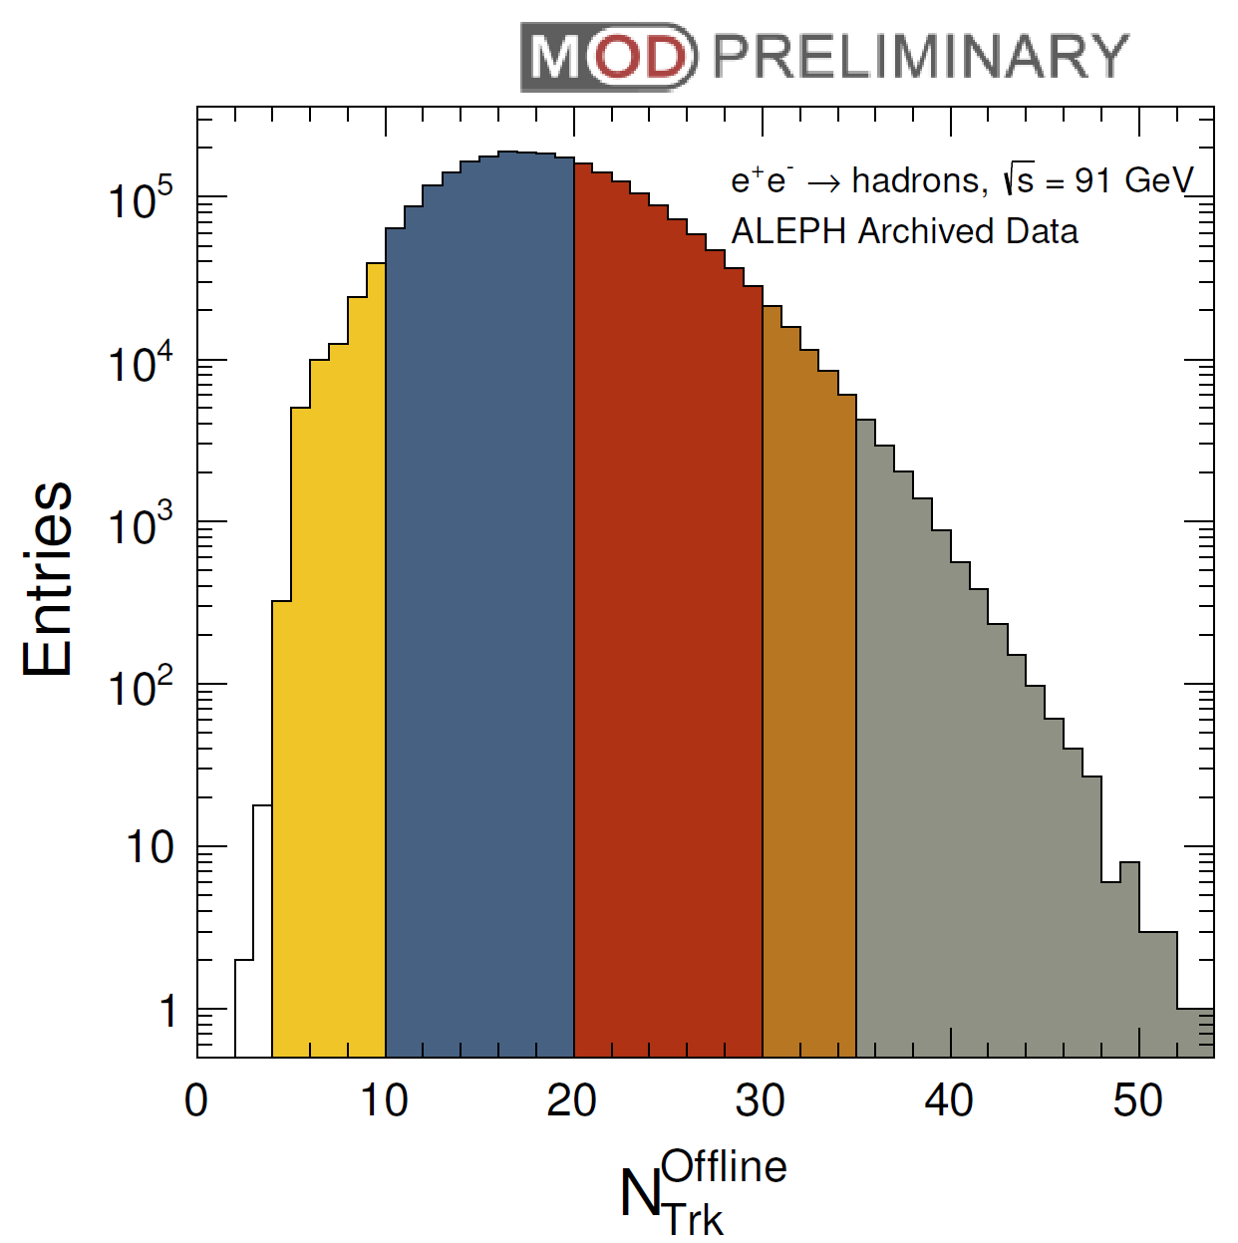
\includegraphics[width=.45\textwidth]{plots/event/nTrkOffline.png}
%\caption{Charged particle multiplicity in ALEPH archived data}
%\label{fig:figure1} 
%\end{center}
%\end{figure}


%%%%%%%%%%%%%%%%%%%%%%%%%%%%%%%%%%%%%%%%%%%%%%%%%%%%%%%%%%%%%%%%%%%%%%%%%%%%%
%\section{\label{sec:datasample}Data Sample and Event Selection}

%\subsection{\label{sec:}ALEPH Detector}
%\subsection{\label{sec:}Event Selection}
%\subsection{\label{sec:}Data Sample and Detector Corrections}

%%%%%%%%%%%%%%%%%%%%%%%%%%%%%%%%%%%%%%%%%%%%%%%%%%%%%%%%%%%%%%%%%%%%%%%%%%%%%
%\section{\label{sec:analysis}Analysis}
Charged particles with transverse momentum $p_{T}>0.2$ GeV/c and $|\eta|<1.74$ are selected for the correlation function analysis. High multiplicity events are sampled using charged particle multiplicity $N$ in each event. The first step in extracting the correlation function was to divide the sample into $N$ bins. For each multiplicity class, ``trigger" particles are defined as charged particles in the selected transverse momentum range. Particle pairs are then formed by associating every trigger particle with the remaining charged particles in the same $p_{\rm T}$ interval as the trigger particle. The per-trigger-particle associated yield is defined as $\frac{1}{N_{\rm trig}}\frac{\rm d^2N^{pair}}{d\Delta\eta  \rm d\Delta\phi}= B(0,0) \times \frac{S(\Delta\eta, \Delta\phi)}{B(\Delta\eta, \Delta\phi)}$, where $N_{trig}$ is the number of trigger particles in the event, $\Delta\eta$ and $\Delta\phi$ are the differences in $\eta$ and $\phi$ of the pair. The signal distribution, $S(\Delta\eta, \Delta\phi)$, is the per-trigger-particle yield of particle pairs in the same event which is defined as $S(\Delta\eta,\Delta\phi) = \frac{1}{N_{trig}}\frac{\rm d^2 N^{\rm same}}{\rm d\Delta\eta \rm d\Delta\phi}$. The mixed-event background distribution, used to account for random combinatorial background, is defined as $B(\Delta\eta,\Delta\phi) = \frac{1}{N_{trig}}\frac{\rm d^2 N^{\rm mix}}{\rm d\Delta\eta \rm d\Delta\phi}$ and is constructed by pairing the trigger particles from two random events in the same event multiplicity interval.
The symbol $N^{mix}$ denotes the number of pairs taken from the mixed event, while $B(0,0)$ represents the mixed-event associated yield for both particles of the pair going in the same direction and thus having full pair acceptance. Therefore, 
the ratio $B(0,0)/B(\Delta\eta,\Delta\phi)$ represents the pair-acceptance correction factor used to derive the corrected per-trigger-particle
associated yield distribution.  The signal and background distributions are first calculated for each event and then averaged over all the events within the track multiplicity class. Simulated events with the PYTHIA event generator (version 6.1 ~\cite{Sjostrand:2000wi}) are used to derive efficiency correction factors for charged particles.

%%%%%%%%%%%%%%%%%%%%%%%%%%%%%%%%%%%%%%%%%%%%%%%%%%%%%%%%%%%%%%%%%%%%%%%%%%%%%
%\section{\label{sec:results}Results}
In Fig.~\ref{fig:figure1}, the two-particle correlation functions from high (N$>$35) multiplicity events are presented using the beam axis as the reference axis for the calculation of $\eta$ and $\phi$ of the charged particles. The dominant features of the correlation function are the jet peak near $(\Delta\eta,\Delta\phi)=(0,0)$ for pairs of particles originating from the same jet and the away-side structure at $\Delta\phi\sim\pi$ for pairs of particles from back-to-back jets. Correlated yields are obtained from an zero-yield-at-minimum (ZYAM) method~\cite{Ajitanand:2005jj} as a function of $|\Delta\phi|$ averaged over $1.6<|\Delta\eta|<3.0$, which are shown in the right panel of Fig.~\ref{fig:figure1}.
Different from the results from pp and pA collisions, no ``ridge"-like structure is found at $\Delta\phi \sim0$. To investigate the collective behavior transverse to the direction of the color string of the outgoing quark and anti-quark pairs from Z decay, the event thrust axis is used to replace the role of the electron beam axis. The charged particle pseudorapidity and polar angles are recalculated with respect to the thrust axis. The obtained correlation functions are shown in Fig.~\ref{fig:figure2}. In the away-side at $\Delta\phi\sim\pi$, the elongated structure is more similar to the ones obtained in pp and pA collisions. The correlated yields as a function of $\Delta\phi$ are consistent with archived simulated PYTHIA events, where no additional final state interactions of the partons are implemented. To suppress the contribution of jet correlations and increase the sensitivity to soft gluon emissions perpendicular to the thrust axis, a pseudorapidity selection of the charged particle $|\eta|<1.6$ is applied. The resulting correlation function and the correlated yields with this selection are shown in Fig.~\ref{fig:figure3}. The observed correlated yields are also consistent with results from simulated PYTHIA events.


\begin{figure}[!htb]
\begin{center}
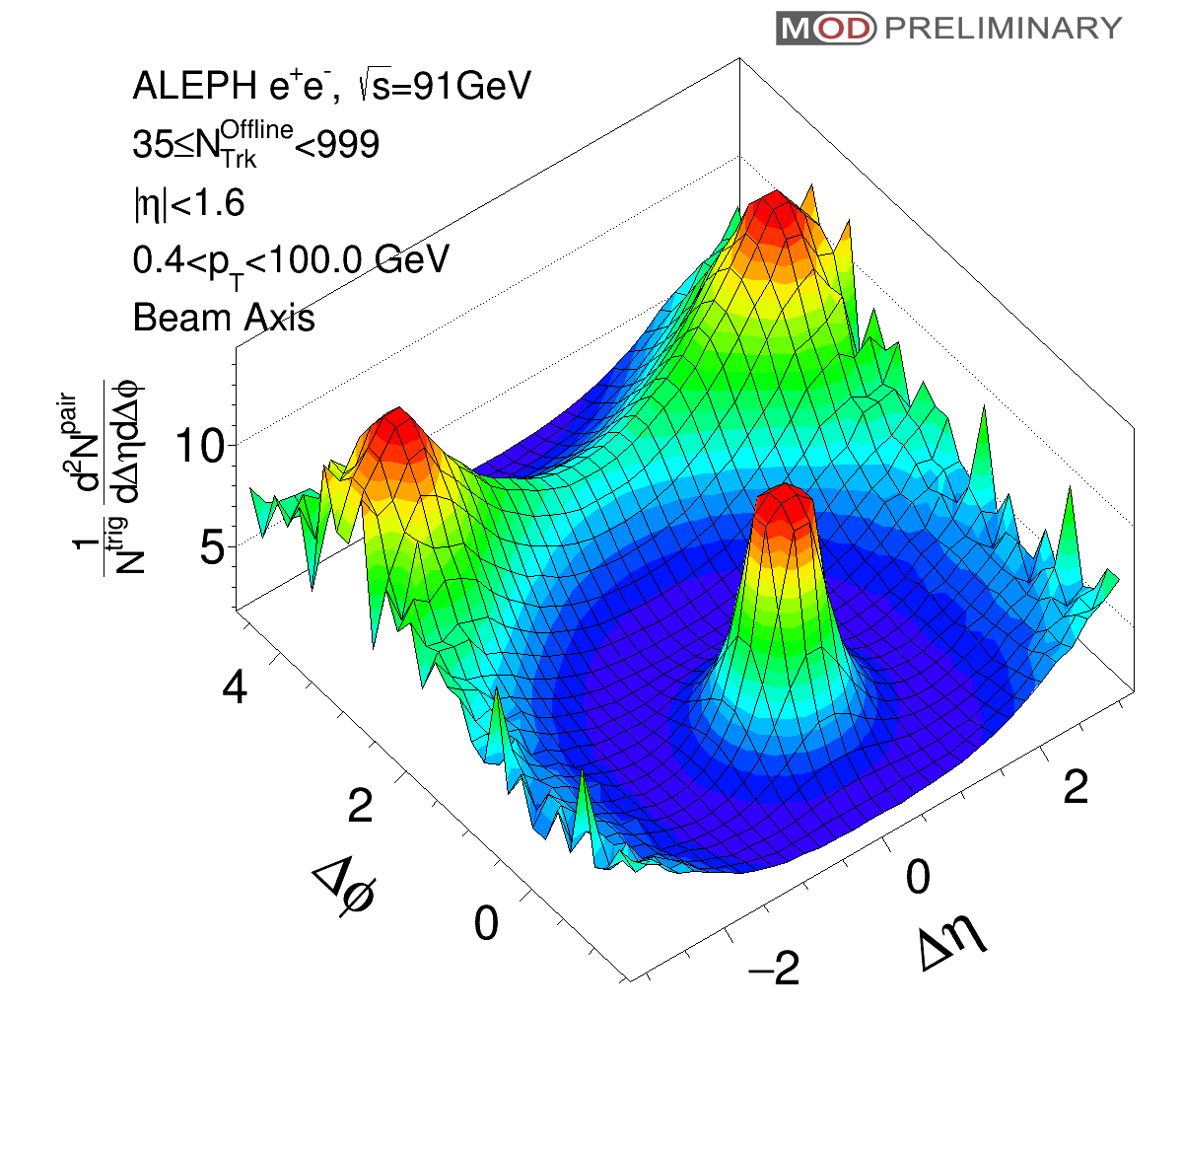
\includegraphics[width=.29\textwidth]{plots/beam/beamAxisAnalysis.png}
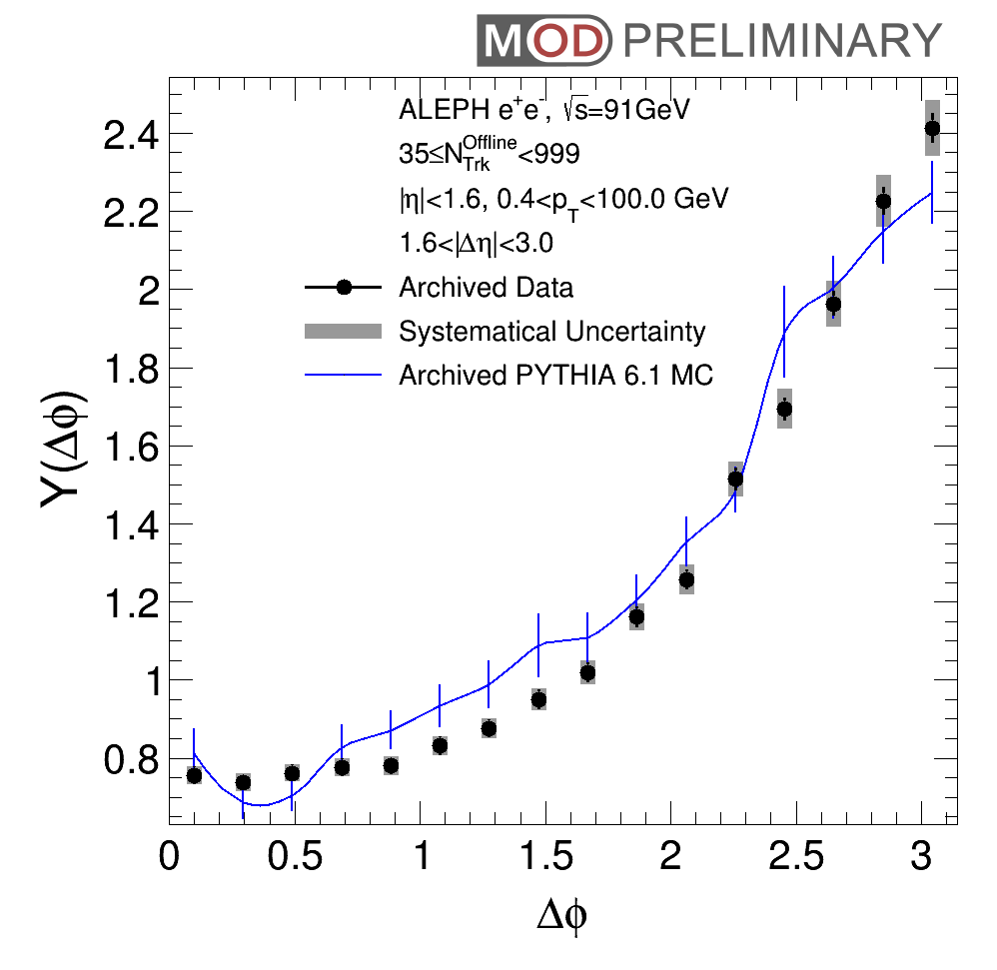
\includegraphics[width=.29\textwidth]{plots/beam/beamAxisAnalysisProjection.png}
\caption{(Left panel) Two-particle correlation functions in $e^{+}e^{-}$ collisions at 91 GeV for events with particle multiplicity $N>$ 35. The sharp near-side peaks from jet correlations have been truncated to better illustrate the structure outside that region. (Right panel) Correlated yield obtained from ZYAM procedure as a function of $|\Delta\phi|$ averaged over $1.6<|\Delta\eta|<3.0$. The error bars correspond to statistical uncertainties, while the shade areas denote the systematic uncertainties.}
\label{fig:figure1} 
\end{center}
\end{figure}

\begin{figure}[!htb]
\begin{center}
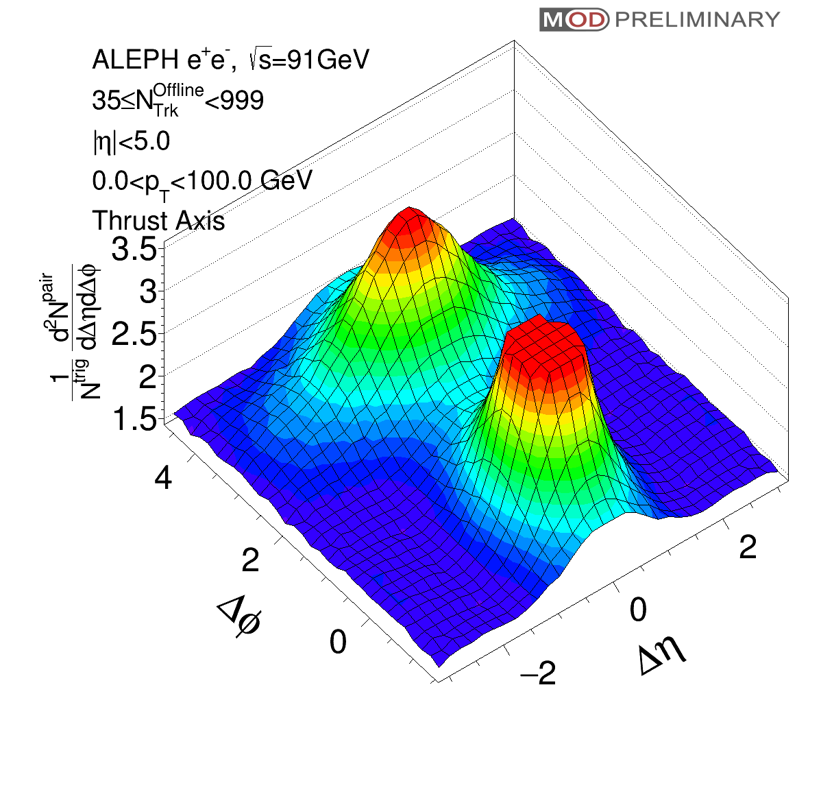
\includegraphics[width=.29\textwidth]{plots/thrust/thrustAxisAnalysis.png}
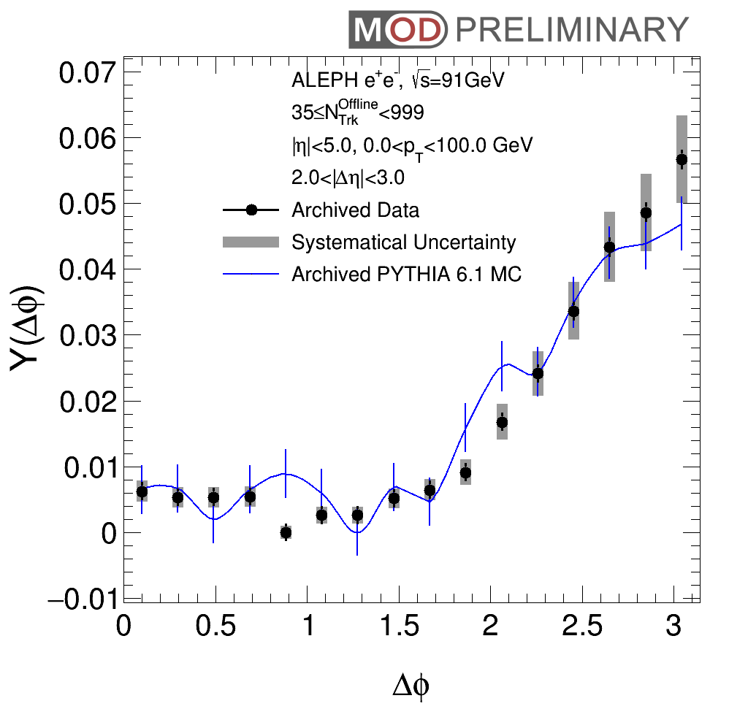
\includegraphics[width=.29\textwidth]{plots/thrust/thrustAxisAnalysisProjection.png}
\caption{(Left panel) Two-particle correlation functions with thrust axis in $e^{+}e^{-}$ collisions at 91 GeV for events with particle multiplicity $N>$ 35. The sharp near-side peaks from jet correlations have been truncated to better illustrate the structure outside that region. (Right panel) Correlated yield obtained from ZYAM procedure as a function of $|\Delta\phi|$ averaged over $1.6<|\Delta\eta|<3.0$. The error bars correspond to statistical uncertainties, while the shade areas denote the systematic uncertainties.}
\label{fig:figure2} 
\end{center}
\end{figure}

\begin{figure}[!htb]
\begin{center}
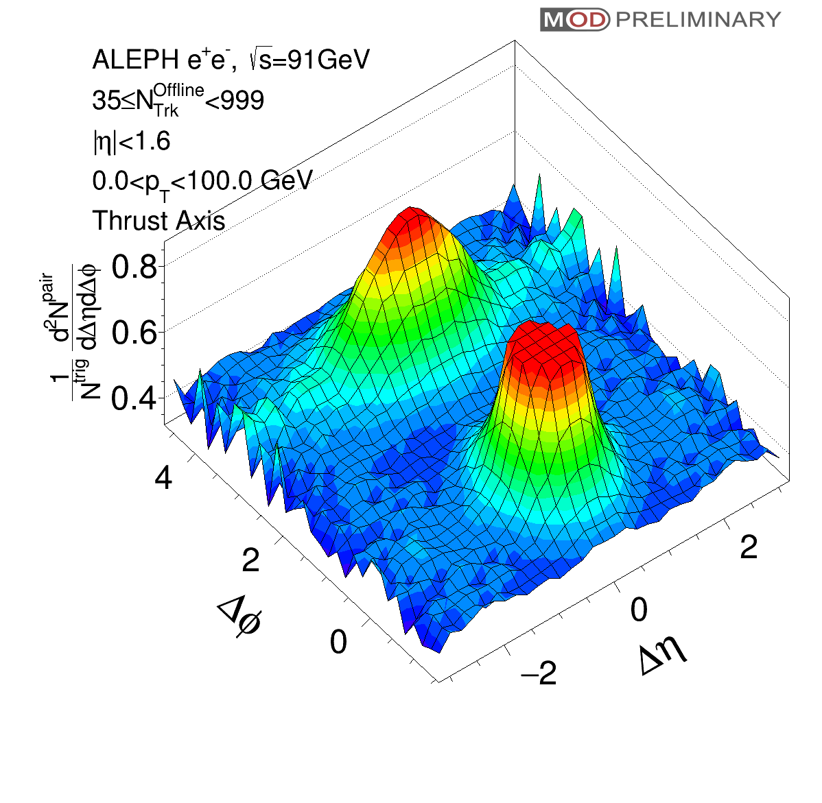
\includegraphics[width=.29\textwidth]{plots/thrustBarrel/thrustAxisBarrelAnalysis.png}
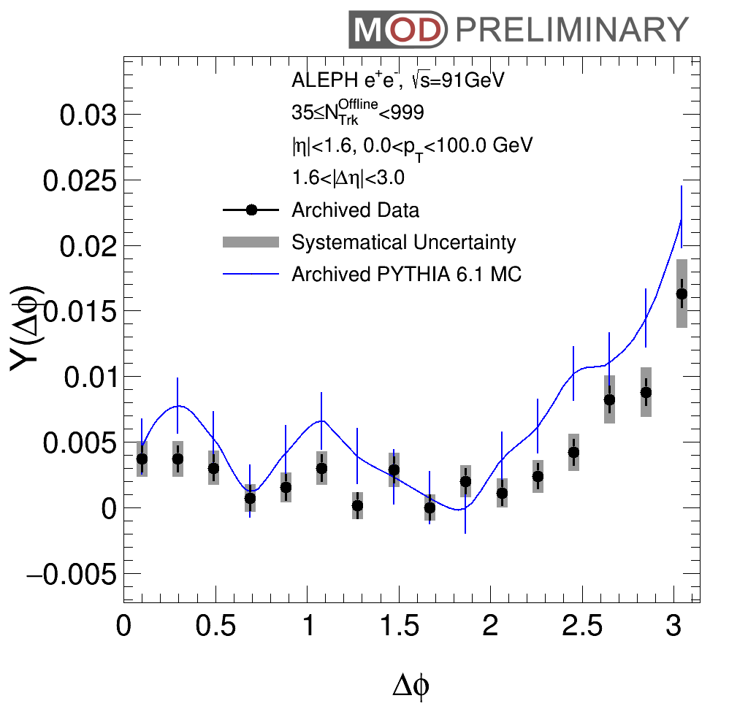
\includegraphics[width=.29\textwidth]{plots/thrustBarrel/thrustAxisBarrelAnalysisProjection.png}
\caption{(Left panel) Two-particle correlation functions with thrust axis in $e^{+}e^{-}$ collisions at 91 GeV for events with particle multiplicity $N>$ 35. Charged particles with $|\eta|<1.6$ are used in the correlation function calculations. The sharp near-side peaks from jet correlations have been truncated. (Right panel) Correlated yield obtained from ZYAM procedure as a function of $|\Delta\phi|$ averaged over $1.6<|\Delta\eta|<3.0$. The error bars correspond to statistical uncertainties, while the shade areas denote the systematic uncertainties.}
\label{fig:figure3} 
\end{center}
\end{figure}



%%%%%%%%%%%%%%%%%%%%%%%%%%%%%%%%%%%%%%%%%%%%%%%%%%%%%%%%%%%%%%%%%%%%%%%%%%%%%
%\section{\label{sec:systematic}Systematic uncertainties}
%Add here discussion of the systematic results

%%%%%%%%%%%%%%%%%%%%%%%%%%%%%%%%%%%%%%%%%%%%%%%%%%%%%%%%%%%%%%%%%%%%%%%%%%%%%
%\section{\label{sec:monteCarlo}Monte carlo comparison}
%Add here discussion of the monte carlo comparisons

%\subsection{\label{sec:LEP2}LEP2}


%%%%%%%%%%%%%%%%%%%%%%%%%%%%%%%%%%%%%%%%%%%%%%%%%%%%%%%%%%%%%%%%%%%%%%%%%%%%%
%\section{\label{sec:summary}Summary}
In summary, the first measurements of two-particle angular correlations for charged particles emitted in $e^+e^-$ collisions at a center-of-mass energy of 91 GeV are presented using archived data collected with the ALEPH detector at LEP. The correlation functions are measured over a broad range of pseudorapidity and azimuthal angle of the charged particles. Those results using either the electron beam axis or the event thrust axis are compared to predictions from the PYTHIA event generator. In contrast to the results from high charged particle multiplicity pp, pA and AA collisions, where long-range correlations with large pseudorapidity gap are observed, no significant enhancement of long-range correlations is observed with respect to PYTHIA predictions, which do not include additional final state interactions of the outgoing partons. Those results serve as an important reference to the
pp, pA and AA collisions.
%%%%%%%%%%%%%%%%%%%%%%%%%%%%%%%%%%%%%%%%%%%%%%%%%%%%%%%%%%%%%%%%%%%%%%%%%%%%%


\begin{acknowledgments}
We wish to acknowledge ......
\dots.
\end{acknowledgments}

\nocite{*}
\bibliography{ridgepaperALEPH}

\end{document}
%
% ****** End of file template.aps ******
